\chapter{Kramer Rate Theory}\label{kramer}
\lhead[\fancyplain{}{\bfseries\thepage}]{\fancyplain{}{\bfseries\rightmark}}
In this Chapter we make a briefly introduction in stochastic process and in Kramer Rate Theory.
\section{Kramer Rate Theory}
We consider the Smoluchowski equation:
\begin{equation}
dx = -V'(x)dt + \sqrt{2T} dw_t
\end{equation}

\begin{figure}
\centering
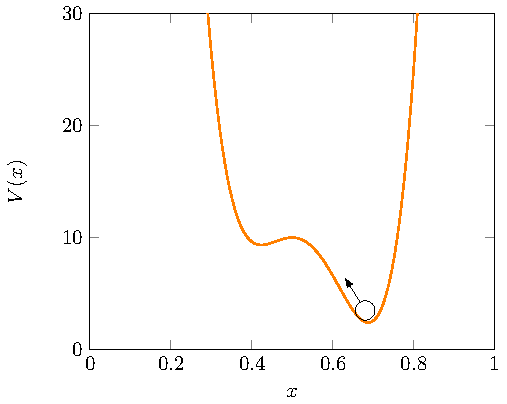
\includegraphics[scale=1.2]{images/kramerwell.pdf}
\caption{\emph{Example of double-well potential.}}
\label{fig:kr}


\end{figure}
where $V(x)$ is a double well potential with $x_a$ and $x_c$ local minima separated by a saddle point $x_b$: To compute the transition probability from the left well to the right well we consider the stationary solution of the Fokker-Planck equation:
\begin{equation}
\frac{\partial \rho}{\partial t } = \frac{\partial}{\partial x} U'(x)\rho + T \frac{\partial ^2 }{\partial x^2} \rho
\end{equation}

with the boundary condition that we have a source in the point $x_{-} < x_a$ and an absorbing boundary at the point $x_{+} > x_c$. We assume that the temperature $T$ is much les of the potential barrier $V_b - V_a$ and we look for a solution that reduces to the form:
$$
e^{-\frac{V(x)}{T}}
$$
in the vicinity of the point $x_a$ that vanishes at the absorbing barrier and gives a constant current $J$ between the two wells. Let
\begin{equation}
\rho(x)=C(x)e^{-\frac{V(x)}{T}}
\end{equation}
and the particle density current $-J=V'(x)\rho + \frac{\partial \rho}{\partial x}T$ reads
$$
V'(x)C(x)e^{-\frac{V}{T}} + C'(x)Te^{-\frac{V}{T}} - V'(x)C(x)e^{-\frac{V}{T}} = -J
$$
so that: 
$$
C'(x) = -\frac{J}{T}e^{\frac{V}{T}}
$$
and we integrate with the condition $C(x_{+}) = 0$:
$$
C(x) = \frac{J}{T}\int_{x}^{x_{+}} e^{\frac{V(y)}{T}}dy
$$


